\chapter{Discrete Fourier Transform}\label{ch:fourier}

\noindent
To begin with, let us review the definition and some properties of Fourier transform since it is confusing in some cases.
The Fourier theorem states that
\begin{equation}\label{eq:fourier_theorem}
f(t) = \frac{1}{2\pi} \int_{-\infty}^\infty \int_{-\infty}^{\infty} f(t^\prime)\, \me^{i\omega(t^\prime-t)} \dd{t}^\prime  \dd{\omega} .
\end{equation}
where the function $f(t^\prime)$ in the right hand side is the same function in the left hand side.  You can express this theorem in two separate integrals.  First, we extract the integral with respect to $t^\prime$ from Eq.(\ref{eq:fourier_theorem}) and define  a  function
\begin{equation}\label{eq:fourier_fwd}
\tilde{f}(\omega) = \int_{-\infty}^{\infty} f(t^\prime)\, \me^{i \omega t^\prime}\, \dd{t}^\prime
\end{equation}
and then we write the theorem  as
\begin{equation}\label{eq:fourier_inv}
f(t) = \frac{1}{2\pi} \int_{-\infty}^\infty \tilde{f}(\omega)\, \me^{-i\omega t}\, \dd{\omega} .
\end{equation}
Equations (\ref{eq:fourier_fwd}) and (\ref{eq:fourier_inv}) are commonly called forward and inverse Fourier transform, respectively.
In Physics $t$ and $\omega$ indicate time and angular frequency.  Therefore, "forward" and "inverse" can be distinguished.  The forward transformation changes the function from the time domain to the frequency domain. There is some confusion regarding the sign on the exponential function.  If $\omega$ in Eq (\ref{eq:fourier_theorem}) is replaced with $-\omega$, the theorem still holds.  That means we could call Eq. (\ref{eq:fourier_inv}) forward transformation and Eq. (\ref{eq:fourier_fwd}) inverse transformation.  In fact,
when we use position $x$ in place of $t$ and wave number $k$ in place of $\omega$, we use the opposite convention of the sign
  
\begin{subequations}
\begin{eqnarray}
\tilde{f}(k)&=&  \int_{-\infty}^{\infty} f(x)\, \me^{- i k x}\, \dd{x} \\
f(x)&=&\frac{1}{2\pi} \int_{-\infty}^\infty \tilde{f}(k)\, \me^{i k x}\, \dd{k}\,.
\end{eqnarray}
\end{subequations}
This expression is more convenient in physics because a traveling wave is mathematically expressed by  $\me^{i(k x - \omega t)}$ where spacial and time domains have the opposite sign.

Mathematically speaking, however, $t$ and $\omega$ are just two different variables.  Apart from the prefactor $1/2\pi$ and the sign of $\omega$ in the exponential function, the two integrals have the identical form. $\tilde{f}(\omega)$ is  Fourier transform of $f(t)$ and $f(t)$ is Fourier transform of $\tilde{f}(\omega)$.  It does not make a sense to call one as forward and the other as inverse. In mathematics literature, the Fourier transform is often defined by
\begin{subequations}\label{eq:fourier_symmetric}
\begin{eqnarray}
\tilde{f}(\omega)&=& \frac{1}{\sqrt{2\pi}} \int_{-\infty}^{\infty} f(t)\, \me^{i \omega t}\, \dd{t} \\
f(t)&=&\frac{1}{\sqrt{2\pi}} \int_{-\infty}^\infty \tilde{f}(\omega)\, \me^{-i\omega t}\, \dd{\omega}\,.
\end{eqnarray}
\end{subequations}
so that the same prefactor appears in both transformation.

In some comunity, yet another expression  
\begin{equation}\label{eq:fourier_fwd_f}
\tilde{f}(\omega) = \int_{-\infty}^{\infty} f(t^\prime)\, \me^{2 \pi i f t^\prime}\, \dd{t}^\prime
\end{equation}
 is used. Then we write the inverse transformation  as
\begin{equation}\label{eq:fourier_inv_f}
f(t) =  \int_{-\infty}^\infty \tilde{f}(\omega)\, \me^{-2 \pi i f t}\, \dd{f} .
\end{equation}
where $f=\omega/2\pi$ is regular frequency.

As you can see slightly different definitions are used in different communities.  Accordingly, Fourier transform programs provided by a computational software package use a different sign convention and a prefactor.  You must check the definition used by the package carefully.
For example, in MATLAB \texttt{fft()} is the forward Fourier transform and \texttt{ifft()} is the inverse Fourier transform.  By default, MATLAB uses Eq. \eqref{eq:fourier_symmetric}.  However, MATLAB provides options to use different definitions.

\section{Discrete Fourier Transform}

If we want to know $\tilde{f}(\omega)$ just for a particular value of $\omega$, the transformation (\ref{eq:fourier_fwd}) is simply an improper integral and thus the numerical methods we studied in Chapter 2 is sufficient.  In general that is not what we want.  We want to know the function $\tilde{f}(\omega)$ for $-\infty < \omega <\infty$. That is a big challenge for digital computers.  If  $t$ is discretized with $N$ points and $\omega$ with $M$ points, the transformation needs the order of $N M$ operations.  In 3 dimensional space, $N$ can be easily $1 \times 10^{6}$.  $M$ is also in the similar order.  Hence, the number operation can be huge.  Fortunately, there is an ingenious method called fast fourier tranform or FFT.  We will briefly study the general aspect of discrete Fourier transform.   The algorithm of FFT will be explained in next section.


First, we need to replace the infinite integration interval $(-\infty, +\infty)$ in Eq. (\ref{eq:fourier_fwd}) with $[-T/2,+T/2]$ where $T>0$ is assumed to be sufficiently large so that $f(t)\approx 0$ for $|t|\ge T/2$.  Second, we introduce discrete time $t_n = n \Delta t$ ($n=-N/2, \cdots, N/2$) where $\Delta t=T/N$.  Then, the transform (\ref{eq:fourier_fwd}) is replaced with  numerical integration
\begin{equation}\label{eq:DFT_fwd}
\tilde{f}(\omega) = \sum_{n=-N/2}^{N/2-1} f(t_n)\, \me^{i n  \omega \Delta t} \, \Delta t\,.
\end{equation}
Here we use the trapezoidal rule for numerical integration.\footnote{It looks like the rectangular rule but recall that when $f(-T/2)=f(T/2)=0$, the rectangular rule is identical to trapezoidal rule.} Since we have chosen $T$ so that $f(-T/2)=f(T/2) \approx 0$, the rectangula rule is OK provided that $\Delta t$ is small enough.  Note that there are $N+1$ sampling points of $t$ but only $N$ rectangles to sum up.  That is why the upper limit of the summation is $N/2-1$.
We need to do the same for $\omega$.  Introducing the integration interval $[-\Omega/2, +\Omega/2]$ and discrete frequency $\omega_m = m \Delta \omega$ ($m=-M/2, \cdots, M/2$) where $\Delta \omega  = \Omega/M$, the inverse transform (\ref{eq:fourier_inv}) is expressed as a numerical integral
\begin{equation}\label{eq:DFT_inv}
f(t) = \frac{1}{2\pi}\sum_{m=-M/2}^{M/2-1} \tilde{f}(\omega_m) \, \me^{-im \Delta \omega t}\, \Delta \omega\,.
\end{equation}

Now, the discrete forms of transformations must consistent with the Fourier theorem. Substituting Eq. (\ref{eq:DFT_fwd}) to Eq. (\ref{eq:DFT_inv}), the discrete version of the Fourier theorem is
\begin{equation}
f(t_k) = \frac{1}{2\pi} \sum_{m=-M/2}^{M/2}\quad \sum_{n=-N/2}^{N/2} f(t_n) \me^{i (n-k) m \Delta \omega \Delta t} \Delta \omega \Delta t.
\end{equation}
\begin{equation}
\tilde{f}(\omega_k) = \frac{1}{2\pi} \sum_{n=-N/2}^{N/2}\quad \sum_{m=-M/2}^{M/2} \tilde{f}(\omega_m) \me^{-i (m-k) n \Delta \omega \Delta t} \Delta \omega \Delta t.
\end{equation}
These equations hold simultaneously  when $N=M$ and $\Delta \omega \Delta t = 2\pi/N$.  Commonly, $\Delta t = T/N$ and $\Delta \omega = 2\pi /T$ are used. The bound of $\omega$ is now $\Omega=2\pi N/T$.  Considering the periodicity of the exponential function, the bound of the summation $(-N/2,N/2-1)$ may be shifted to $(0,N-1)$. 

In practice, the choice of $T$ is sometime tricky.  Normally, we choose $T$ such that $f(T/2) \approx 0$ and $N$ such that the resolution $\Delta t=T/N$ is small enough.  However, we also need a reasonable resolution of frequency $\Delta\omega=2\pi/T$.  If $T$ is too small, the resolution of the frequency becomes poor.  Therefore, a larger $T$ is better for the frequency.  On the other hand, if $T$ is large, $N$ has to be large so that the resolution of time is fine enough. (See Example \ref{ex:fft_gaussian}.)

In summary, the discrete version of Fourier transforms (DFT) are defined by
\begin{subequations}\label{eq:DFT}
\begin{eqnarray}
\tilde{f}_m &=& T \left ( \frac{1}{N}\sum_{n=0}^{N-1} f_n\, \me^{2 \pi i m n / N} \right )\label{eq:DFT_fwd2}\\
f_n &=& \frac{1}{T} \left ( \sum_{m=0}^{N-1} \tilde{f}_m\, \me^{- 2 \pi i n m /N} \right )\label{eq:DFT_inv2}
\end{eqnarray}
\end{subequations}
where function values are abbreviated with $f_n \equiv f(t_n)$ and $\tilde{f}_m\equiv \tilde{f}(\omega_m)$.
An important consequence of the discretization is that the discretized functions are periodic even when the original functions are not.
Explicitly writing it, 
\begin{subequations}
\begin{eqnarray}
f_{n+N} = f_n \qquad &\text{or}& \qquad  f(t+T)=f(t) \\
\tilde{f}_{n+N}=\tilde{f}_n \qquad &\text{or}& \qquad  \tilde{f}(\omega+\Omega) = \tilde{f}(\omega).
\end{eqnarray}
\end{subequations}

DFT can be expressed in a matrix form,
\begin{equation}\label{eq:DFT_matrix}
\tilde{\mathbf{f}} = \mathcal{F}\, \mathbf{f}, \qquad \mathbf{f} = \mathcal{F}^{-1}\, \tilde{\mathbf{f}}
\end{equation}
where the matrix is defined by
\begin{equation}
\mathcal{F}_{mn} = \frac{T}{N}  \me^{2\pi i m n/N}, \quad n,m = 0, \cdots, N-1
\end{equation}
and the functions are expressed as vectors
\begin{equation}
\mathbf{f} = \begin{bmatrix}
f_1 \\ f_2 \\ \vdots \\ f_N
\end{bmatrix}, \qquad
\tilde{\mathbf{f}} = \begin{bmatrix}
\tilde{f}_1 \\ \tilde{f}_2 \\ \vdots \\ \tilde{f}_N
\end{bmatrix}
\end{equation}
The multiplication of a matrix and a vector involves $N^2$ of multiplications and $N^2$ of additions, which can be too large if we need to perform Fourier transform many times.

\section{Fast Fourier Transform}

An remarkable algorithm was developed in 19 century but not very popular until modern computers appeared in 1960's.
It allows us to perform Fourier transform with only $N \log_2 N$ operations instead of $N^2$.  When $N=1024$,
$N \log_2 N = 10240$ where as $N^2 \approx 1 \times 10^{6}$ which is 100 times large. The saving is even bigger as $N$ increases.
The algorithm, known as Fast Fourier Transform (FFT), is very popular and widely used in a variety of applications in science, engineering and beyond.\footnote{FFT is built in many computational environments such as MATLAB.  FFT libraries are available for almost any computer language, among them Fast Fourier Transform in the West (FFTW) is popular and available for a variety of languages including C/C++, Fortran, Python, Java, etc.  See \url{www.fftw.org}.}

The FFT utilizes the structure the matrix $\mathcal{F}$.  Consider $N=8$ for example, the matrix is 
\begin{eqnarray}
\mathcal{F} &=& \frac{T}{8}
\begin{bmatrix}
1 &               1 &               1 &               1 &               1 &               1 &               1 &               1 \\
1 &  \me^{i  \pi/4} & \me^{i  2\pi/4} & \me^{i  3\pi/4} & \me^{i  4\pi/4} & \me^{i  5\pi/4} & \me^{i  6\pi/4} & \me^{i  7\pi/4} \\
1 &  \me^{i 2\pi/4} & \me^{i  4\pi/4} & \me^{i  6\pi/4} & \me^{i  8\pi/4} & \me^{i 10\pi/4} & \me^{i 12\pi/4} & \me^{i 14\pi/4} \\
1 &  \me^{i 3\pi/4} & \me^{i  6\pi/4} & \me^{i  9\pi/4} & \me^{i 12\pi/4} & \me^{i 15\pi/4} & \me^{i 18\pi/4} & \me^{i 21\pi/4} \\
1 &  \me^{i 4\pi/4} & \me^{i  8\pi/4} & \me^{i 12\pi/4} & \me^{i 16\pi/4} & \me^{i 20\pi/4} & \me^{i 24\pi/4} & \me^{i 28\pi/4} \\
1 &  \me^{i 5\pi/4} & \me^{i 10\pi/4} & \me^{i 15\pi/4} & \me^{i 20\pi/4} & \me^{i 25\pi/4} & \me^{i 30\pi/4} & \me^{i 35\pi/4} \\
1 &  \me^{i 6\pi/4} & \me^{i 12\pi/4} & \me^{i 18\pi/4} & \me^{i 24\pi/4} & \me^{i 30\pi/4} & \me^{i 36\pi/4} & \me^{i 42\pi/4} \\
1 &  \me^{i 7\pi/4} & \me^{i 14\pi/4} & \me^{i 21\pi/4} & \me^{i 28\pi/4} & \me^{i 35\pi/4} & \me^{i 42\pi/4} & \me^{i 49\pi/4} 
\end{bmatrix}\label{eq:Fmatrix1}\\
 &=& \frac{T}{8}
\begin{bmatrix}
1 &               1 &               1 &               1 &               1 &               1 &               1 &               1 \\
1 & \me^{ i  \pi/4} &               i &-\me^{-i  \pi/4} &              -1 &-\me^{ i  \pi/4} &              -i & \me^{-i  \pi/4} \\
1 &               i &              -1 &              -i &               1 &               i &              -1 &              -i \\
1 &-\me^{-i  \pi/4} &              -i & \me^{ i  \pi/4} &              -1 & \me^{-i  \pi/4} &               i &-\me^{ i  \pi/4} \\
1 &              -1 &               1 &              -1 &               1 &              -1 &               1 &              -1 \\
1 &-\me^{ i  \pi/4} &               i & \me^{-i  \pi/4} &              -1 & \me^{ i  \pi/4} &              -i &-\me^{-i  \pi/4} \\
1 &              -i &              -1 &               i &               1 &              -i &              -1 &               i \\
1 & \me^{-i  \pi/4} &              -i &-\me^{ i  \pi/4} &              -1 &-\me^{-i  \pi/4} &               i & \me^{ i  \pi/4} 
\end{bmatrix}\label{eq:Fmatrix2}
\end{eqnarray}
In the second matrix (\ref{eq:Fmatrix2}), the exponential functions are simplified as much as possible.  You can see easily that Matrix (\ref{eq:Fmatrix2}) is much simpler than Matrix (\ref{eq:Fmatrix1}). You notice that many matrix elements share the same value. A simple trick reveals further the simplicity of the transformation matrix. First, we reorder the elements of the vector in a ``magic'' order:
\begin{equation}
\mathbf{f}^\prime = 
\begin{bmatrix}
f_0 \\ f_4 \\ f_2\\ f_6\\ f_1\\ f_5\\ f_3\\ f_7 
\end{bmatrix}, \qquad \text{and}
\qquad
\tilde{\mathbf{f}}^\prime = 
\begin{bmatrix}
\tilde{f}_0 \\ \tilde{f}_4 \\ \tilde{f}_2\\ \tilde{f}_6\\ \tilde{f}_1\\ \tilde{f}_5\\ \tilde{f}_3\\ f_7
\end{bmatrix}
\end{equation}
and then reorder the columns and rows of (\ref{eq:Fmatrix2}) accordingly so that Eq. (\ref{eq:DFT_matrix}) holds.
\begin{equation}
\mathcal{F}^\prime = \frac{T}{8}
\begin{bmatrix}
1 &  1 &               1  &                1 &                1 &                1 &                1 &                1 \\
1 &  1 &               1  &                1 &               -1 &               -1 &               -1 &               -1 \\
1 &  1 &              -1  &               -1 &                i &                i &               -i &               -i \\
1 &  1 &              -1  &               -1 &               -i &               -i &                i &                i \\
1 & -1 &               i  &               -i &  \me^{ i  \pi/4} & -\me^{ i  \pi/4} & -\me^{-i  \pi/4} &  \me^{-i  \pi/4} \\
1 & -1 &               i  &               -i & -\me^{ i  \pi/4} &  \me^{ i  \pi/4} &  \me^{-i  \pi/4} & -\me^{-i  \pi/4} \\
1 & -1 &              -i  &                i & -\me^{-i  \pi/4} &  \me^{-i  \pi/4} &  \me^{ i  \pi/4} & -\me^{ i  \pi/4} \\
1 & -1 &              -i  &                i &  \me^{-i  \pi/4} & -\me^{-i  \pi/4} & -\me^{ i  \pi/4} &  \me^{ i  \pi/4} 
\end{bmatrix}
\end{equation}
Writing  $\tilde{\mathbf{f}}^\prime=\mathcal{F}^\prime \mathbf{f}^\prime$ explicitly,
\begin{subequations}
\begin{eqnarray}
\tilde{f}_0 &=& [(f_0+f_4) + (f_2+f_6)] + [(f_1+f_5) + (f_3+f_7)] \\
\tilde{f}_4 &=& [(f_0+f_4) + (f_2+f_6)] - [(f_1+f_5) + (f_3+f_7)] \\
\tilde{f}_2 &=& [(f_0+f_4) - (f_2+f_6)] +i[(f_1+f_5) - (f_3+f_7)] \\
\tilde{f}_6 &=& [(f_0+f_4) - (f_2+f_6)] -i[(f_1+f_5) - (f_3+f_7)] \\
\tilde{f}_1 &=& [(f_0-f_4) + i(f_2-f_6)] + [\me^{ i\pi/4} (f_1-f_5) - \me^{-i\pi/4} (f_3-f_7)]\\
\tilde{f}_5 &=& [(f_0-f_4) + i(f_2-f_6)] - [\me^{ i\pi/4} (f_1-f_5) - \me^{-i\pi/4} (f_3-f_7)]\\
\tilde{f}_3 &=& [(f_0-f_4) - i(f_2-f_6)] - [\me^{-i\pi/4} (f_1-f_5) - \me^{ i\pi/4} (f_3-f_7)]\\
\tilde{f}_7 &=& [(f_0-f_4) - i(f_2-f_6)] + [\me^{-i\pi/4} (f_1-f_5) - \me^{ i\pi/4} (f_3-f_7)],
\end{eqnarray}
\end{subequations}
we clearly see the regularity in the matrix.
Now look at the additions in the regular parentheses $(\cdots)$.  Many additions are identical.  In fact, there are 32 additions but only 8 different ones. We can reduce the computation by factor 4.  Furthermore, the additions inside the square bracket $[\cdots]$ are duplicated in the following line. Hence, we reduce the  calculation by factor 2.  For a large matrix we can save a lot of computation time.  

The permutation of rows and columns gives us the clear picture of this redundant additions.  How do we determine the permutation?  It turns out to be very simple. Express the element indexes in binary, e.g. $3=011$, then reverse the order of the bits, $011 \rightarrow 110$ which is $7$.  Then, we swap column 3 and 7.  Figure \ref{fig:bit_reversed_order} illustrates the bit reversed order.

The above algorithm of FFT works only when $N=2^k$.  In modern FFT libraries other values of $N$ can be used.  However, the power of 2 gets the best performance.  If we have a data set whose size is not the power of two, we can just add 0 to the data set until the total number of data becomes the power of 2.  This zero padding does not cause a problem since the data outside the bounds is already assumed to be zero.


\begin{figure}
\centering
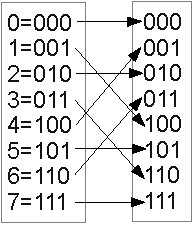
\includegraphics[width=1in]{11.fft/bit_reversed_order.pdf}
\caption{Bit reversed order for $N=8$.}\label{fig:bit_reversed_order}
\end{figure}

\section{Remarks on the use of canned routines in MATLAB and Python}

The detail use of the FFT package strongly depends on their implementation.  It is important to read the manual carefully before using it. The most popular FFT package is FFTW\cite{FFTW97} which earned J. H. Wilkinson Prize for Numerical Software in 1999. MATLAB is based on FFTW.  Numpy package in Python includes its own FFT based on
Cooley and Tukey algorithm\cite{Cooley1965} which is well explained in Numerical Recipes\cite{numerical_recipes}.
PyFFTW, which calls FFTW, is currently being deveopled.
MATLAB and Numpy have build-in functions \texttt{fft()} and \texttt{ifft()} which work in similar way. \texttt{fft()} computes
\begin{equation}\label{eq:matlab_fft}
F_k = \sum_{m=0}^{N-1} f_m \exp(-i \frac{2\pi\, k\, m}{N})
\end{equation}
and \texttt{ifft()}
\begin{equation}\label{eq:matlab_ifft}
f_m = \frac{1}{N} \sum_{k=0}^{N-1} F_k \exp(i \frac{2\pi\, k\, m}{N})
\end{equation}
using the FFT algorithm. 

The users must prepare the input data set $\{f_m\}$ suitable for their application and converts output data $\{F_k\}$ to suitable form by reordering and a multiply constant. Some key points we need to know are given below.

\subsection{Forward or Backward Transformation}

Apart from the factor $T/N$ and $1/T$, the difference between forward and backward transformation is the sign in the exponent. It is just the convention issue.  FFTW, used $\me^{-i\omega t}$ as forward, which is opposite to ours.    My forward transformation may be your backward transformation. We just have to use a routine which has a desired sign.   MATLAB and Numpy use the same convention as FFTW.

\subsection{Prefactor in front of the Summation}

FFTW does not multiply $T/N$ in  Eq. (\ref{eq:DFT_fwd2})  nor $1/T$ in Eq. (\ref{eq:DFT_inv2}).  It is up to the users to multiply an appropriate prefactors.  This means that the output of the FFTW does not satisfy the Fourier theorem (\ref{eq:fourier_theorem}) unless $1/N$ is multiplied by the user.  MATLAB and Numpy use a different convention.  The inverse FFT function \texttt{ifft()} defined by Eq. \eqref{eq:matlab_ifft}, differs  from Eq. (\ref{eq:DFT_fwd2}) by factor $T$ and the forward FFT function \texttt{fft()} defined by Eq. \eqref{eq:matlab_fft} differs from Eq. (\ref{eq:DFT_inv2}) by factor $1/T$.  The user must multiply these factors manually. 

\subsection{Input/Output Format: Bit Reversed or Not}

Most FFT routines carry out the bit reversal permutation internally. So, the users don't have to do it by themselves.  However, the order of output depends on the FFT routines. Some FFT routines return the results in the original order but others in the bit reversed order. Advanced packages allow the users to specify the output order.  Why do we want the result in bit reversed order? In some cases, we repeat FFT many times but we need only the final output.  Therefore, there is no need to change the order back and forth every time.  If the bit-reversed order is kept during the repeated FFT, computing time is significantly saved. By default, MATLAB and Numpy return the data in the regular order.

\subsection{Input/Output format: Periodicity}

Even when the output is not in the bit reversed order, the order of input/output data is often very confusing.  Recall that we replaced $\sum_{n=-N/2}^{N/2-1}$ with $\sum_{n=0}^{N-1}$.
FFT assumes that $t=0, \Delta t, 2\Delta t, \cdots, (N-1)\Delta t$ and that the function values are stored in this order. There is no negative $t$!.  Suppose that we have a function data $f_n$ for $n=0, \cdots, N-1$ with $t_n = (n-N/2) \Delta t$.  Although $t$ begins with a negative value $-N/2$, FFT doesn't care about it and assume that the first data $f_0$ is at $t=0$. That is obviously wrong.  Therefore, we need to change the order of the input data.  Since the functions in DFT are periodic, we can add the period $T$ to $t$ without changing the function value.  For $t<0$, use $\mathbf{f}(t+T)$. Now the function is evaluated at positive time only.  In summary, the input data must be reordered as follows.
\begin{equation}
\mathbf{f}^\textsc{raw data}=
\begin{bmatrix}
f_0\\
\vdots\\
f_{N/2}\\
f_{N/2+1}\\
\vdots\\
f_{N-1}
\end{bmatrix} \quad \Longrightarrow \quad
\mathbf{f}^\textsc{input} =
\begin{bmatrix}
f_{N/2+1} \\
\vdots \\
f_{N-1} \\
f_0\\
\vdots\\
f_{N/2}
\end{bmatrix}
\end{equation}

Similarly, the order of the output data is shifted in the same way as the input order.
Usually, you want to get a function $\tilde{f}(\omega)$ from $-\Omega/2$ to $\Omega/2$.  The output from FFT is not like that.  The first half of the data is for $\omega = 0$ to $\omega=\Omega/2$ and the latter half begins with $\omega=-\Omega/2$   to $\omega=-\Delta \omega$.  The user must reordered the output before plotting it as following:
\begin{equation}
\tilde{\mathbf{f}}^\textsc{output} = 
\begin{bmatrix}
\tilde{f}_0\\
\vdots\\
\tilde{f}_{N/2}\\
\tilde{f}_{N/2+1}\\
\vdots\\
\tilde{f}_{N-1}
\end{bmatrix} \quad \Longrightarrow \quad
\tilde{\mathbf{f}}^\textsc{plot} =
\begin{bmatrix}
\tilde{f}_{N/2+1}\\
\vdots\\
\tilde{f}_{N-1}\\
\tilde{f}_{0}\\
\vdots\\
\tilde{f}_{N/2}
\end{bmatrix}
\end{equation}

Both MATLAB and Numpy provide functions \texttt{fftshift()} and \texttt{ifftshift()} to carryout the above transformation.  The following example explains how to prepare the input data and recover the output you need.

\bigskip
\noindent
\begin{example}[Foureir Transform of a Gaussian Function]\label{ex:fft_gaussian}

\medskip
\noindent
Let us compute the Fourier transform of a normalized Gaussian function
\begin{equation}
f(t) = \frac{1}{\sqrt{\pi}} \me^{-t^2}.
\end{equation}
The analytic solution is given by
\begin{equation}
\tilde{f}(\omega) = \frac{1}{\sqrt{\pi}} \int_{-\infty}^\infty \me^{-t^2} \me^{i \omega t} \dd{t}  = \me^{-\omega^2/4}
\end{equation}

\begin{figure}
\centering
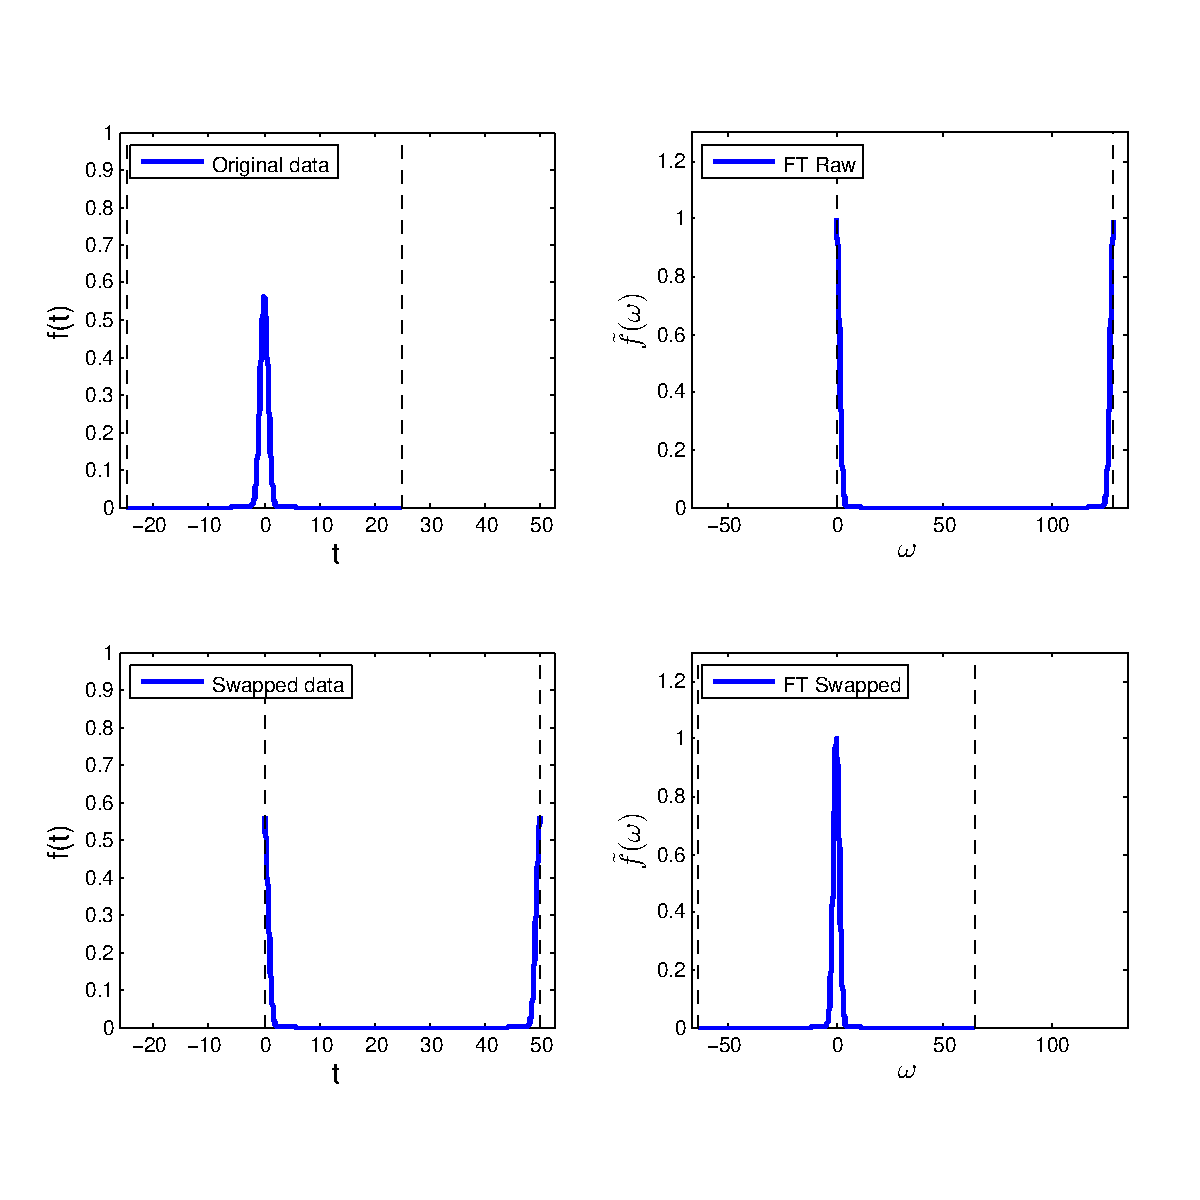
\includegraphics[width=4in]{11.fft/fft_gaussian_order.pdf}
\caption{Fast Fourier transform of a gaussian function. \textit{Top left}: The original function value centered around $t=0$.  The dashed lines indicate the lower and upper bounds at $\pm T/2$.  \textit{Bottom left}:  The lower half ($t<0$) of the function is shifted by $T$.  Now the bounds are $(0,T)$ indicaed by the dashed line. \textit{Top right}: Fourier transform of the Gaussian generated by MATLAB function \texttt{ifft()}.  The lower and upper bounds of the frequency is 0, $\Omega=2\pi N/T$ indicated by the dashed line. \textit{Bottom right}:
The upper half of the data is shifted by $-\Omega$.  Now, the Fourier transform is peaked around $\omega=0$.}
\label{fig:fft_gaussian_order}
\end{figure}

First, we have to decide the parameter values. $T=50$ and $N=1024=2^{10}$ makes time resolution $\Delta t \approx 0.05$ fine enough. The function value at the bound $f(\pm T/2) \approx 10^{-272}$ seems unnecessarily too small.  A smaller $T$ could be used.  However, the resolution of the frequency is $\Delta \omega = 2\pi/T \approx 0.1$, barely small enough.  Therefore, we cannot reduce $T$.

A raw data set $\mathbf{f}$ is created using a domain $-T/2 < t < T/2$, which is plotted in Fig \ref{fig:fft_gaussian_order} (top left).  Then, the lower half of the data is shifted by $T$.  In the program, we just swap the lower and upper half of the column vector.   The resulting function is plotted in Fig \ref{fig:fft_gaussian_order} (bottom left).  MATLAB's function \texttt{ifft()} calculate our forward Fourier transform (\ref{eq:DFT_fwd2}).  The raw output is plotted in Fig \ref{fig:fft_gaussian_order} (top right). The frequency domain is bounded by $0$ and $\Omega=2 \pi/T$, indicated by the dashed line.  It is difficult to see the profile. Therefore, we swap the lower and upper half of the output array to get a normal plot for $-\Omega/2 < \omega < \Omega/2$, which is plotted in Fig \ref{fig:fft_gaussian_order} (bottom right).
It is still difficult to see the detail because the result is nearly zero for the most part.  These zero regions are needed to keep the resolution of $t$ small enough.  Finally, we zoom into the important region.  In Fig \ref{fig:fft_gaussian}, the final result and exact solution are compared.  The agreement is nearly perfect.  

\begin{figure}
\centering
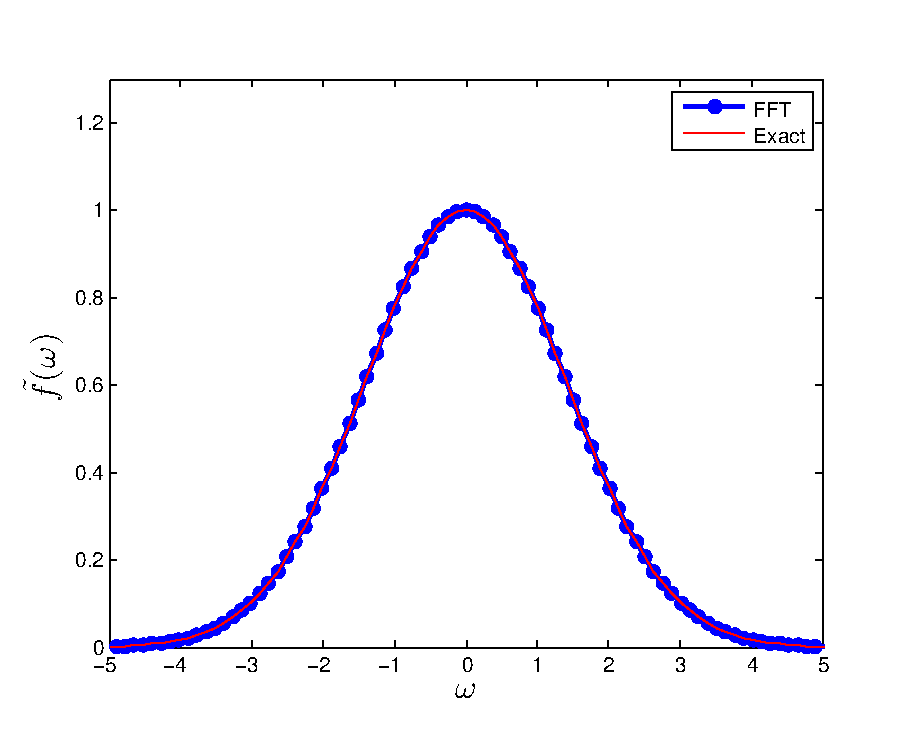
\includegraphics[width=2.5in]{11.fft/fft_gaussian.pdf}
\caption{Fourier transform of the Gaussian distribution, which is again Gaussian in the Fourier space. The output of FFT agrees well with the exact solution.}\label{fig:fft_gaussian}
\end{figure}
\end{example}

\noindent
\section{Applications in Physics}

\subsection{Laplacian operator}\label{sec:fft_laplacian}

The Laplacian operator $\nabla^2$ is everywhere in physics.  We try to evaluate one-dimensional Laplacian acting on a function using FFT.
Consider
\begin{equation}
g(x) = \frac{\md^2}{\md x^2} f(x).
\end{equation}
Introducing the Fourier transform of $f(x)$, the above equation can be written as
\begin{eqnarray}
g(x) &=&  \frac{\md^2}{\md x^2} \frac{1}{2\pi} \int_{-\infty}^\infty \tilde{f}(k) \me^{i k x} \md k \nonumber \\
&=& \frac{1}{2\pi} \int_{-\infty}^\infty (-k^2) \tilde{f}(k) \me^{i k x} \md k \\
\end{eqnarray}
The last integral is just an inverse Fourier transform of $-k^2 \tilde{f}(k)$.  To solve this problem, we use FFT  twice.  First, we transform the original function $f(x)$ to $\tilde{f}(k)$ and multiply $-k^2$ to it.  Then, Fourier transform back to the original space.  The result is $g(x)$.  

As an example, we apply the Laplacian to a Gaussian function $f(x)=\me^{-x^2}/\sqrt{\pi}$.  The analytic solution is $g(x) = (4x^2-2) \me^{-x^2}$.  The following code uses MATLAB's \texttt{fft()} and \texttt{ifft}.  Note that we don't have to multiply prefacters.  When both forward and inverse transformations are carried out, they canceled out. If you use FFTW, you must divide the final output by $N$.  Figure \ref{fig:fft_laplacian} plots the result which is in a good agreement with the analytic solution.


\begin{figure}
\centering
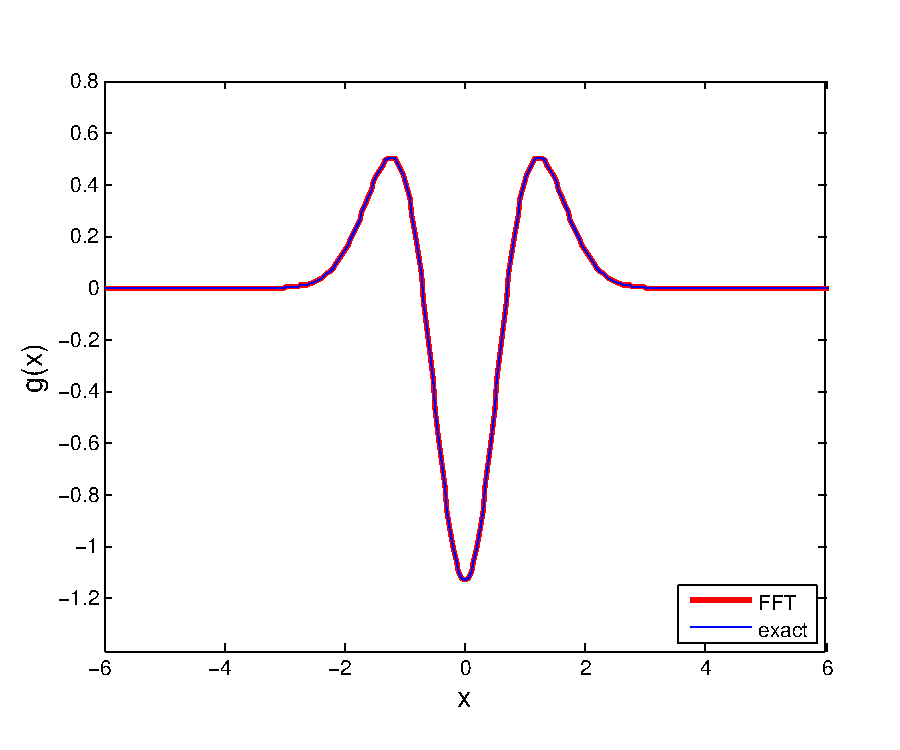
\includegraphics[width=2.5in]{11.fft/fft_laplacian.pdf}
\caption{Laplacian by FFT: Output of Example \ref{ex:fft_gaussian}.}
\label{fig:fft_laplacian}
\end{figure}

\subsection{Correlation Functions}

The convolution of functions $f(t)$ and $g(t)$ is defined by
\begin{equation}
(f \circ g) (\tau) \equiv \int_{-\infty}^{\infty} f(t) g(\tau-t) \dd{t}
\end{equation}
This kind of integral is used as a definition of autocorrelation functions
\begin{equation}
\langle x(\tau) x(0) \rangle \equiv \int_{-\infty}^{\infty} x(t) x(t+\tau) \dd{t}.
\end{equation}

The convolution can be evaluated by using FFT twice.
Introducing Fourier transform of $x(t)$,
\begin{eqnarray}
\langle x(\tau) x(0) \rangle &=& \int_{-\infty}^{\infty} \left ( \frac{1}{2\pi}\int_{-\infty}^{\infty} \tilde{x}^*(\omega) \me^{i \omega t} \dd{\omega} \right ) \left ( \frac{1}{2\pi} \int_{-\infty}^{\infty} \tilde{x}(\omega^\prime) \me^{-i \omega^\prime (t+\tau)} \dd{\omega}^\prime \right ) \dd{t} \nonumber\\
&=& \frac{1}{2\pi} \int_{-\infty}^{\infty} \dd{\omega} \int_{-\infty}^{\infty} \dd{\omega}^\prime \tilde{x}^*(\omega)  \tilde{x}(\omega^\prime) \me^{-i \omega^\prime \tau} 
\left (\frac{1}{2\pi} \int_{-\infty}^{\infty} \me^{i(\omega-\omega^\prime) t} \dd{t} \right ) \nonumber\\
&=&
\frac{1}{2\pi}\int_{-\infty}^{\infty} \dd{\omega} \int_{-\infty}^{\infty} \dd{\omega}^\prime \tilde{x}^*(\omega)  \tilde{x}(\omega^\prime) \me^{-i \omega^\prime \tau} 
\delta (\omega-\omega^\prime) \nonumber\\
&=& \frac{1}{2\pi}\int_{-\infty}^{\infty}  
 |\tilde{x}(\omega)|^2 \me^{-i \omega \tau} \dd{\omega}
 \label{eq:conv_fourier}
\end{eqnarray}
where we used a delta function 
\begin{equation}
\delta(\omega) = \frac{1}{2\pi} \int_{-\infty}^{\infty} \me^{i \omega t } \dd{t}.
\end{equation}
The last expression of Eq. (\ref{eq:conv_fourier}) is just an inverse Fourier transform.  The function $|\tilde{x}(\omega)|^2$ is called power spectrum of the temporal function $x(t)$ and the relation between the convolution and the power spectrum is known as Wiener-Khinchin theorem.

To compute the autocorrelation function, compute the Fourier transform $\tilde{x}(\omega)$, evaluate the power spectrum $|\tilde{x}(\omega)|^2$ , and then transform it back to the $t$ domain. The result is the autocorrelation function.
We will use this method in Chap XX to investigate the correlation in stochastic processes.

\subsection{Spectral Analysis}

In Sections 7.5.2 and 9.3.1, we investigated coupled harmonic oscillators.  First, we obtained the equilibrium positions of oscillators using a root finding method. Then, we calculated the eigenfrequencies of the normal modes by solving an eigenvalue problem.  Here, we try to find the eigenfrequencies by solving Newton's equation (9.24) directly. We use the Verlet algorithm to integrate the equation of motion. Initially all oscillators are assumed to be at the equilibrium position. Then, we kick one of the mass at $t=0$.  The other masses are initially at rest.  The trajectories of the oscillators are plotted in the left panel of Fig \ref{fig:coupled_springs_speactra}.  It looks random and difficult to see any periodic motion.  Therefore, it is impossible to identify the frequencies of the normal mode.  Since we know the normal modes from the previous investigation in Sec 9.3.1.  we could excite just one of them.  Then, we will be able to see a periodic motion.  However, there is a better way.

Writing the trajectory as a linear combination of normal modes:
\begin{equation}
\mathbf{x}(t) = \sum_{i=1}^{3} c_i \mathbf{u}_i \me^{i \omega_i t}
\end{equation}
where $\mathbf{u}_i$ and $\omega_i$ are $i$th normal mode and its frequency.  The complex coefficient $c_i$ is determined by the initial condition.  Now, we calculate the Fourier transform of $\mathbf{x}(t)$.
\begin{equation}
\tilde{\mathbf{x}}(\omega) = \sum_{i=1}^{3} c_i \mathbf{u}_i \int_{-\infty}^{\infty} \me^{i (\omega_i - \omega) t} \dd{t}
= \sum_{i=1}^{3} 2\pi c_i \mathbf{u}_i \delta(\omega-\omega_i).
\end{equation}
This result suggests that the Fourier transform of the trajectory has sharp peaks at the eigenfrequencies. However, we don't have a data for the entire time.  Suppose we have a trajectory from $t=0$ to $t=T$ and calculate ``Fourier transform'' using FFT.  Since the trajectory is not zero after $t=T$, this is not a true Fourier transformation. This ``limited'' Fourier transformation misses some long time behaviors. However, it captures short time behavior correctly.  More precisely, the resolution of $\omega$ domain is limited by $\Delta \omega = 2\pi/T$. We cannot see any fine structure smaller than $\Delta \omega$.  For example the width of peaks cannot be smaller than $\Delta \omega$.  Anys slow oscillation whose frequency smaller than $\Delta \omega$ will not be detected by the FFT.  However, if $\Delta \omega < \omega_i <\Omega$, we will be able to identify the peaks. If the peak is not sharp enough, just calculate the trajectory a little longer. As $T$ increases, the peaks become sharper.

The right panel of Fig. \ref{fig:coupled_springs_speactra} show the power spectra. The total period $T=200$ provides a fine resolution of $\Delta \omega\approx 0.03$, small enough to build sharp peaks.  All three eigenfrequencies are clearly identifiable and they match well to the values obtained from the eigenvalue analysis in Sec. 9.3.1. 

\begin{figure}
\centering
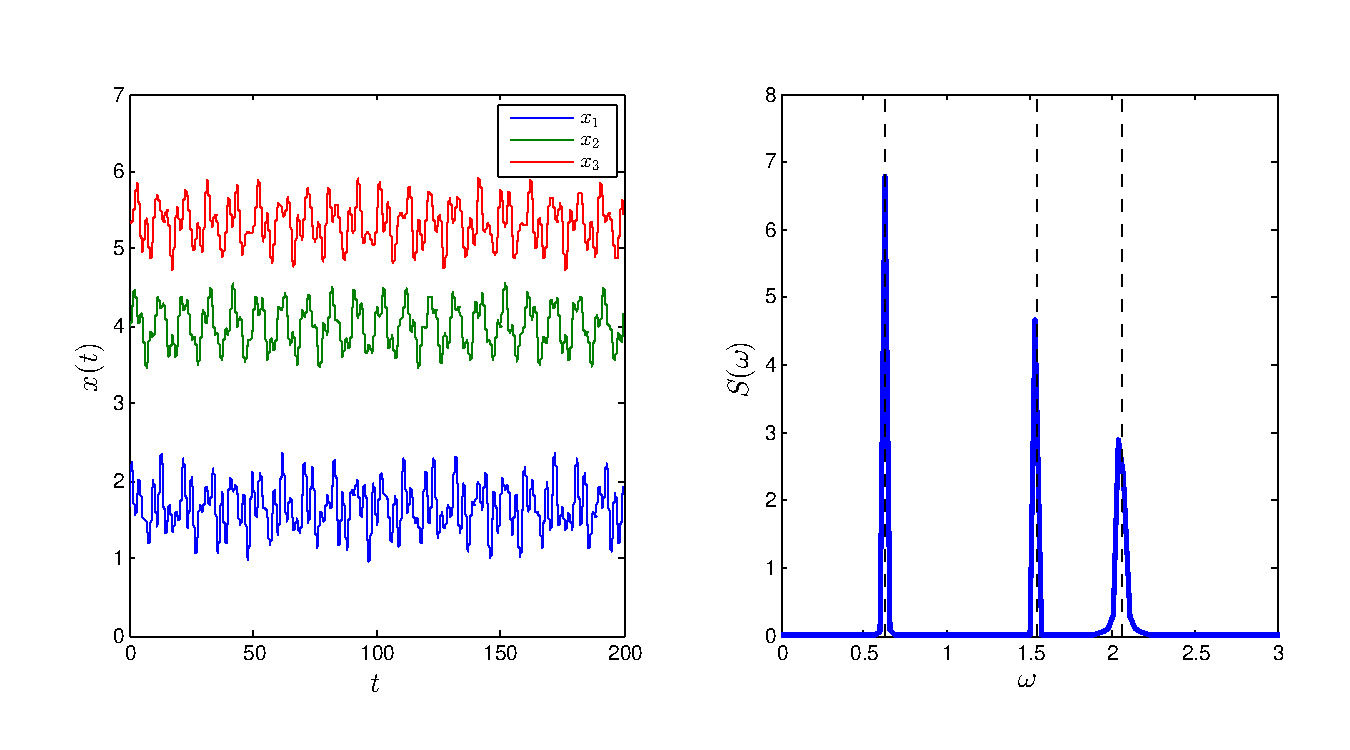
\includegraphics[width=4.5in]{11.fft/coupled_springs_spectra.pdf}
\caption{Normal modes of coupled oscillators by spectral analysis. \textit{Left}:  Trajectories of each oscillators. It looks quite random.  However, they are just a combination of three periodic motion.  \textit{Right} Power spectrum of the trajectory.  Three peaks corresponding to eigenfrequencies are sharp and clear.  The dashed lines indicates the eigenfrequencies obtained by eigenvalue anaysis in Sec. 9.3.1.  They all match to the peak positions.}\label{fig:coupled_springs_speactra}
\end{figure}

\subsection{Wave Function in Momentum Space}

In quantum mechanics, the probability to find the particle in a region between $x$ and $x+\md x$ is given by 
\begin{equation}
|\psi(x)|^2 \md x
\end{equation}
where $\psi(x)$ is a wave function in the position space.
Similarly the probability that the momentum of the particle is between $p$ and $p + \md p$ is given by
\begin{equation}
|\tilde{\psi}(p)|^2 \md p
\end{equation}
where $\tilde{\psi}(p)$ is a wave function in the momentum space. These two wave functions are related by
\begin{equation}
\psi(x) = \frac{1}{\sqrt{2\pi \hbar}} \int_{-\infty}^{\infty} \tilde{f}(p) \me^{i p x/\hbar} \md p
\end{equation}
This is nothing but a Fourier transform except for the prefactors.  It is more convenient to use wave number $k=p/\hbar$. \footnote{In atomic units $\hbar=1$. Then $p=k$.}

Now consider the energy eigenstates of a quantum harmonic oscillator.  Here, we show the wave functions of the lowest three states using a normalized coordinate $x$ (assume that $m \omega/\hbar = 1$),
\begin{subequations}
\begin{eqnarray}
\psi_0(x) &=& \frac{1}{\sqrt{ \sqrt{\pi}}} \me^{-x^2/2} \\
\psi_1(x) &=& \frac{2}{\sqrt{2\sqrt{\pi}}} x \me{-x^2/2}\\
\psi_2(x) &=& \frac{1}{\sqrt{2\sqrt{\pi}}} (2 x^2 -1) \me^{-x^2/2}
\end{eqnarray}
\end{subequations}
we have already calculated the Fourier transform the ground state in Example 10.1.  Program XXX computes the wave functions in momentum space and plot them.  The result is plotted in Fig \ref{fig:momentum_psi}.
In classical mechanics the lowest energy state corresponding to the particle is still at $x=0$.  In quantum case, the mean momentum is zero as the plot shows.  However, the probability to find a particle with non-zero momentum is not small due to the uncertainty principle.  As energy increases, the second and third states allow higher momentum.  Note that the mean momentum is zero even for the higher energy states since the particle moves both directions and thus the momentum cancels out. 

\begin{figure}
\centering
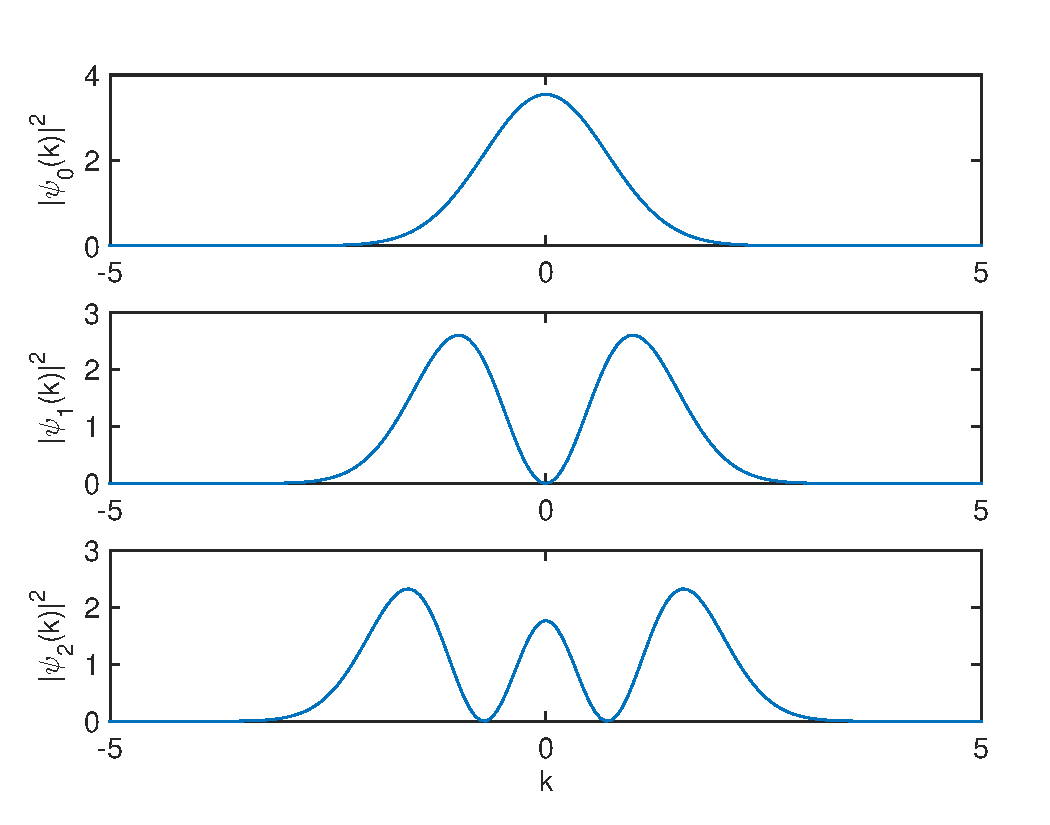
\includegraphics[width=3.5in]{11.fft/momentum_psi.pdf}
\caption{The probability density in momentum space for a quantum harmonic oscillator}
\label{fig:momentum_psi}
\end{figure}

\newpage
\section{Problems}

\begin{enumerate}[labelwidth=0.5cm,labelindent=0cm,leftmargin=*,label=\bfseries \thechapter.\arabic*,align=left]

\item \textbf{Power Spectrum of Chaotic Motion}

\medskip
\noindent
Solve the Lorentz equations
\begin{subequations}
\begin{eqnarray}
\dot{x} &=& \sigma (y-x)\\
\dot{y} &=& x (\rho - z) \\
\dot{z} &=& x y - \beta z
\end{eqnarray}
\end{subequations}
for Parameter values $\sigma=10$, $\beta=8/3$, and $\rho=28$.  Plot the power spectra of $x(t)$ and $y(t)$ and $z(t)$.  Do you see any peak?
Do you see any distinct pattern in the spectrum?  
\newpage

\end{enumerate}

\newpage
\section*{MATLAB Source Codes}
\addcontentsline{toc}{section}{\protect\numberline{}MATLAB Source Codes}


\bigskip
\noindent
\program
\label{prog:fft_gauss}
\footnotesize
\begin{lstlisting}[language=matlab]
%**************************************************************************
%*     Example 11.1                                                       *
%*     filename: ch11pr01.m                                               *
%*     program listing number: 11.1                                       *
%*                                                                        *
%*     This program calculates the Fourier transform of Gaussian.         *
%*                                                                        *
%*     Uses MATLAB function ifft()                                        *
%*                                                                        *
%*     Programed by Ryoichi Kawai for Computational Physics Course.       *
%*     Last modification:  02/08/2015.                                    *
%**************************************************************************
clear all

% control parameters
N=1024;
T=50; %size of time domain
W=2*pi*N/T; % size of the frequency domain
dt=T/N;  % resolution int
dw=2*pi/T; % resolution in omega


t0=[-N/2:N/2-1]*dt;% original time
t1=[0:N-1]*dt;% shifted time
w0=[-N/2:N/2-1]*dw; %original frequeny 
w1=[0:N-1]*dw; %shifted frequency


% function in normal order
f0=exp(-t0.^2)/sqrt(pi);

% function in swapped order
f1(1:N/2)=f0(N/2+1:N);
f1(N/2+1:N)=f0(1:N/2);

% FFT
g1=ifft(f1)*T;% do not forget to multiply T

% swap back to normal order
g0(1:N/2)=g1(N/2+1:N);
g0(N/2+1:N)=g1(1:N/2);

% analytic FT
g2=exp((-w0.^2)/4);

subplot(2,2,1)
p=plot(t0,f0);
set(p,'linewidth',2);
hold on

axis([-T/2*1.05 T*1.05 0 1.0]);
legend('Original data')
legend('location','northwest')
xlabel('t','fontsize',14)
ylabel('f(t)','fontsize',14)
q=plot([-T/2,-T/2],[0,1],'--',[T/2,T/2],[0,1],'--');
set(q,'color','black')
hold off

subplot(2,2,3)
p=plot(t1,f1);
set(p,'linewidth',2);
axis([-T/2*1.05 T*1.05 0 1.0]);
legend('Swapped data')
legend('location','northwest')
xlabel('t','fontsize',14)
ylabel('f(t)','fontsize',14)
hold on
q=plot([0,0],[0,1],'--',[T,T],[0,1],'--');
set(q,'color','black')
hold off

subplot(2,2,2)
p=plot(w1,real(g1));
set(p,'linewidth',2');
axis([-W/2*1.05 W*1.05 0 1.3])
legend('FT Raw')
legend('location','northwest')
xlabel('$\omega$','Interpreter','LaTex','fontsize',14)
ylabel('$\tilde{f}(\omega)$','Interpreter','LaTex','fontsize',14)
hold on
q=plot([0,0],[0,1.3],'--',[W,W],[0,1.3],'--');
set(q,'color','black')
hold off

subplot(2,2,4)
p=plot(w0,g0);
set(p,'linewidth',2');
axis([-W/2*1.05 W*1.05 0 1.3])
legend('FT Swapped')
legend('location','northwest')
xlabel('$\omega$','Interpreter','LaTex','fontsize',14)
ylabel('$\tilde{f}(\omega)$','Interpreter','LaTex','fontsize',14)
hold on
q=plot([-W/2,-W/2],[0,1.3],'--',[W/2,W/2],[0,1.3],'--');
set(q,'color','black')
hold off

figure
p=plot(w0,g0,'-o',w0,g2);
axis([-5 5 0 1.3])
set(p(1),'linewidth',2')
set(p(2),'color','red')
legend('FFT','Exact')
xlabel('$\omega$','Interpreter','LaTex','fontsize',16)
ylabel('$\tilde{f}(\omega)$','Interpreter','LaTex','fontsize',16)
\end{lstlisting}
\normalsize

%\ruleend
\bigskip
\noindent
\program
\label{prog:fft_laplace}
\footnotesize
\begin{verbatim}
%**************************************************************************
%*     Example 11.2                                                       *
%*     filename: ch11pr02.m                                               *
%*     program listing number: 11.2                                       *
%*                                                                        *
%*     This program calculates the fourier transform of the second order  *
%*     derivative.                                                        *
%*                                                                        *
%*     Uses MATLAB function ifft() and fft()                              *
%*                                                                        *
%*     Programed by Ryoichi Kawai for Computational Physics Course.       *
%*     Last modification:  02/08/2015.                                    *
%**************************************************************************
clear all;

% control parameters
N=1024;
L=50; %size of time domain
K=2*pi*N/L; % size of the frequency domain
dx=L/N;  % resolution int
dk=2*pi/L; % resolution in wave number

x0=[-N/2:N/2-1]*dx;% original time
x1=[0:N-1]*dx;% shifted time
k0=[-N/2:N/2-1]*dk; %original frequeny 
k1(1:N/2)=k0(N/2+1:N);
k1(N/2+1:N)=k0(1:N/2);

f0=exp(-x0.^2)/sqrt(pi); % function in normal order

f1(1:N/2)=f0(N/2+1:N); % function in swapped order
f1(N/2+1:N)=f0(1:N/2);

% FFT
F1=ifft(f1);        % prefactor not need this time
F1=-F1.*(k1.^2);    % because we perform both forward
g1=fft(F1);         % and inverse transformation.

g0(1:N/2)=g1(N/2+1:N); % swap back to normal order
g0(N/2+1:N)=g1(1:N/2);

g2=exp(-x0.^2)/sqrt(pi).*(4*x0.^2-2); % analytic FT

p=plot(x0,real(g0),x0,g2);
set(p(1),'linewidth',2,'color','red')
set(p(2),'color','blue')
axis([-6 6 -1.4 0.8])
xlabel('x','fontsize',14)
ylabel('g(x)','fontsize',14)
legend('FFT','exact')
legend('location','southeast')
\end{verbatim}
\normalsize

\ruleend
\bigskip
\noindent
\program
\label{prog:fft_powerspectrum}
\footnotesize
\begin{verbatim}
%**************************************************************************
%*     Section 11.4.3                                                     *
%*     filename: ch11pr03.m                                               *
%*     program listing number: 11.3                                       *
%*                                                                        *
%*     This program calculates the power spectrum of coupled oscillators. *
%*                                                                        *
%*     Uses MATLAB function fft()                                         *
%*                                                                        *
%*     Programed by Ryoichi Kawai for Computational Physics Course.       *
%*     Last modification:  02/08/2015.                                    *
%**************************************************************************
clear all

% system parameters
m=[2,4,3];
k=[2,4,4,2];
L=[1,2,1,2,8];
K=[[k(1)+k(2),-k(2),0];[-k(2),k(2)+k(3),-k(3)];[0,-k(3),k(3)+k(4)]];
b=[k(1)*L(1)-k(2)*L(2); k(2)*L(2)-k(3)*L(3);k(3)*L(3)+k(4)*(L(5)-L(4))];
M=[[1/m(1),0,0];[0,1/m(2),0];[0,0,1/m(3)]];

% initial conditions
x0=[5/3;4;16/3]; % at the equilibrium
v0=[1,0,0];

% control parameters
T=200;
N=4096;
dt=T/N;
dw=2*pi/T;
w=linspace(0,N-1,N)*dw;

% First we calculate the trajectory of oscillators
x(1:3,1)=x0;
v(1:3,1)=v0;
t(1)=0;
% 1st step (Euler step)
x(:,2) = x(:,1)+v(:,1)*dt;
t(2)=t(1)+dt;

% Verlet algorithm
for i=3:N
    f = -K*x(:,i-1)+b;
    x(:,i)=2*x(:,i-1)-x(:,i-2)+(M*f)*dt^2;
    v(:,i-1)=(x(:,i)-x(:,i-2))/(2*dt);
    t(i)=t(1)+(i-1)*dt;
end

% Now, we analyze the trajectories.
X=x(1,:)-x0(1); % deviation form the equilibrium
y=fft(X(1,:))/T; % Fourer transform
S = abs(y(1,:).^2); % power spectrum

Figure1=figure(1);clf;
set(Figure1,'defaulttextinterpreter','latex');
subplot(1,2,1)
plot(t,x(1,:),t,x(2,:),t,x(3,:))
xlabel('$t$','fontsize',14,'interpreter','latex')
ylabel('$x(t)$','fontsize',14,'interpreter','latex')
axis([0 T 0 7])
h=legend('$x_1$','$x_2$','$x_3$');
set(h,'Interpreter','latex')

subplot(1,2,2)
r=plot(w,S);
axis([0 3 0 8])
xlabel('$\omega$','fontsize',14,'interpreter','latex')
ylabel('$S(\omega)$','fontsize',14,'interpreter','latex')
set(r,'linewidth',2)
hold on
q=plot( [2.056127, 2.056127], [0, 8], '--',...
      [1.540700, 1.540700], [0, 8], '--',...
      [0.631338, 0.631338], [0, 8], '--');
set(q,'color','black')
hold off
\end{verbatim}
\normalsize

\ruleend
\bigskip
\noindent
\program
\label{prog:fft_powerspectrum}
\footnotesize
\begin{verbatim}
%**************************************************************************
%*     Section 11.4.4                                                     *
%*     filename: ch11pr04.m                                               *
%*     program listing number: 11.4                                       *
%*                                                                        *
%*     This program calculates the probability distribution of a harmonic *
%*     oscillator in the momentum spapce.
%*                                                                        *
%*     Uses MATLAB function ifft()                                        *
%*                                                                        *
%*     Programed by Ryoichi Kawai for Computational Physics Course.       *
%*     Last modification:  02/08/2015.                                    *
%**************************************************************************
clear all

% control parameters
N=1024;
X=100; %size of position space
K=2*pi*N/X; % size of momentum space
dx=X/N;  % resolution int
dk=2*pi/X; % resolution in omega


x0=[-N/2:N/2-1]*dx;% original time
x1=[0:N-1]*dx;% shifted time
k0=[-N/2:N/2-1]*dk; %original frequeny 
k1=[0:N-1]*dk; %shifted frequency

% function in normal order
psix0=exp(-x0.^2/2)/sqrt(sqrt(pi));
psix1=2*x0.*exp(-x0.^2/2)/sqrt(2*sqrt(pi));
psix2=(2*x0.^2-1).*exp(-x0.^2/2)/sqrt(2*sqrt(pi));


f(1:N/2)=psix0(N/2+1:N); % function in swapped order
f(N/2+1:N)=psix0(1:N/2);
g=ifft(f)*X;% do not forget to multiply T
psik0(1:N/2)=g(N/2+1:N);% swap back to normal order
psik0(N/2+1:N)=g(1:N/2);

f(1:N/2)=psix1(N/2+1:N); % function in swapped order
f(N/2+1:N)=psix1(1:N/2);
g=ifft(f)*X;% do not forget to multiply T
psik1(1:N/2)=g(N/2+1:N);% swap back to normal order
psik1(N/2+1:N)=g(1:N/2);

f(1:N/2)=psix2(N/2+1:N); % function in swapped order
f(N/2+1:N)=psix2(1:N/2);
g=ifft(f)*X;% do not forget to multiply T
psik2(1:N/2)=g(N/2+1:N);% swap back to normal order
psik2(N/2+1:N)=g(1:N/2);


subplot(3,1,1)
p1=plot(k0(N/4:3*N/4),abs(psik0(N/4:3*N/4)).^2);
ylabel(texlabel('|psi_0(k)|^2'))
subplot(3,1,2)
p2=plot(k0(N/4:3*N/4),abs(psik1(N/4:3*N/4)).^2);
ylabel(texlabel('|psi_1(k)|^2'))
subplot(3,1,3)
p3=plot(k0(N/4:3*N/4),abs(psik2(N/4:3*N/4)).^2);
ylabel(texlabel('|psi_2(k)|^2'))
xlabel('k')
hold off
\end{verbatim}
\normalsize

\ruleend

\bigskip
\noindent
\section*{Python Source Codes}
\addcontentsline{toc}{section}{\protect\numberline{}Python Source Codes}
\setcounter{program}{0}

\bigskip
\noindent
\program
\footnotesize
\begin{verbatim}
#!/usr/bin/env python3
# -*- coding: utf-8 -*-
"""
%**************************************************************************
%*     Example 11.1                                                       *
%*     filename: ch11pr01.py                                              *
%*     program listing number: 11.1                                       *
%*                                                                        *
%*     This program calculates the fourier transform of Gaussian.         *
%*                                                                        *
%*     Uses Numpy fft package                                             *
%*                                                                        *
%*     Programed by Ryoichi Kawai for Computational Physics Course.       *
%*     Last modification:  02/18/2017.                                    *
%**************************************************************************
"""
import numpy as np
import matplotlib.pyplot as plt

# control parameters
N=1024

# Setting time domain
T=50.   # size of time domain
dt=T/N  # time interval
tmin=-T/2.
tmax=tmin+dt*(N-1)
t0=np.linspace(tmin,tmax,N)    # original time
t1=np.linspace(0.0,dt*(N-1),N) # fft ordered time

# setting frequency domain
W=2.0*np.pi*N/T # size of the frequency domain
dw=W/N          # frequency resolution
wmin=-W/2.0
wmax=wmin+dw*(N-1)
w0=np.linspace(wmin,wmax,N)     # frequency domain we want
w1=np.linspace(0.0,dw*(N-1),N)  # fft frequency domain

# original Gaussian function in time domain
f0=np.exp(-t0**2)/np.sqrt(np.pi)
# function in fft order
f1=np.fft.fftshift(f0)

# FFT from time to frequency domain in  ffto order
g1=np.fft.ifft(f1)*T  # do not forget to multiply T

# Get the normal frequenx=cy domain order
g0=np.fft.ifftshift(g1)

# analytic FT
g2=np.exp((-w0**2)/4.0)

plt.figure(figsize=(12,10))
plt.subplot(2,2,1)
plt.plot(t0,f0,'-r',label=r'original input',linewidth=2)
plt.plot([-T/2,-T/2],[0,1],'--k')
plt.plot([T/2,T/2],[0,1],'--')
plt.axis([-T/2*1.05, T*1.05, 0.0, 1.0])
plt.legend(loc=2)
plt.xlabel(r'$t$',fontsize=14)
plt.ylabel(r'$f(t)$',fontsize=14)

plt.subplot(2,2,3)
plt.plot(t1,f1,'-r',label='fft input',linewidth=2)
plt.plot([0,0],[0,1],'--k')
plt.plot([T,T],[0,1],'--k')
plt.axis([-T/2*1.05, T*1.05, 0.0, 1.0])
plt.legend(loc=2)
plt.xlabel(r'$t$',fontsize=14)
plt.ylabel(r'$f(t)$',fontsize=14)

plt.subplot(2,2,2)
plt.plot(w1,np.real(g1),'-r',label='fft output',linewidth=2)
plt.plot([0,0],[0,1.3],'--k')
plt.plot([W,W],[0,1.3],'--k')
plt.axis([-W/2*1.05, W*1.05, 0.0, 1.3])
plt.legend(loc=2)
plt.xlabel(r'$\omega$',fontsize=14)
plt.ylabel(r'$\tilde{f}(\omega)$',fontsize=14)

plt.subplot(2,2,4)
plt.plot(w0,g0,'-r',label='desired output',linewidth=2)
plt.plot([-W/2,-W/2],[0,1.3],'--k')
plt.plot([W/2,W/2],[0,1.3],'--k')
plt.axis([-W/2*1.05, W*1.05, 0.0, 1.3])
plt.legend(loc=2)
plt.xlabel(r'$\omega$',fontsize=14)
plt.ylabel(r'$\tilde{f}(\omega)$',fontsize=14)
plt.show()

plt.figure(figsize=(6,5))
plt.plot(w0,g0,'-or',label='FFT',linewidth=2)
plt.plot(w0,g2,'-k',label='Exact',linewidth=2)
plt.xlabel(r'$\omega$',fontsize=14)
plt.ylabel(r'$\tilde{f}(\omega)$',fontsize=14)
plt.show()
\end{verbatim}
\normalsize

\ruleend

\bigskip
\noindent
\program
\footnotesize
\begin{verbatim}
#!/usr/bin/env python3
# -*- coding: utf-8 -*-
"""
%**************************************************************************
%*     Example 11.2                                                       *
%*     filename: ch11pr02.py                                              *
%*     program listing number: 11.2                                       *
%*                                                                        *
%*     This program calculates the fourier transform of the second order  *
%*     derivative.                                                        *
%*                                                                        *
%*     Uses Numpy FFT package                                             *
%*                                                                        *
%*     Programed by Ryoichi Kawai for Computational Physics Course.       *
%*     Last modification:  02/18/2017.                                    *
%**************************************************************************
"""
import numpy as np
import matplotlib.pyplot as plt

# control parameters
N=1024

# position domain
X=50.  # size of position domain
dx=X/N   # position interval
xmin=-X/2.
xmax=xmin+dx*(N-1)
x0=np.linspace(xmin,xmax,N)      # position space in natural order
x1=np.linspace(0.0,dx*(N-1),N)   # position space in fft order

# momentum domain
K=2.0*np.pi*N/X  # size of the momentum domain
dk=K/N           # resolution in momentum space
kmin=-K/2.
kmax=kmin+dk*(N-1)
k0=np.linspace(kmin,kmax,N)     # momentum space in natural order
k1=np.fft.fftshift(k0)          # momentum space in shifted order

f0=np.exp(-x0**2)/np.sqrt(np.pi) # input in natural order
f1=np.fft.fftshift(f0)           # input in fft order

# FFT from position to momentum domain
F1=np.fft.fft(f1)   # prefactor not need this time
F1=-F1*(k1**2)      # because we perform both forward
g1=np.fft.ifft(F1)  # and inverse transformation.
g0=np.fft.ifftshift(g1) # output in natural order

g2=np.exp(-x0**2)/np.sqrt(np.pi)*(4.0*x0**2-2.0)  # analytic FT

plt.figure(figsize=(6,5))
plt.plot(x0,np.real(g0),'-or',label='FFT')
plt.plot(x0,g2,'-b',label='exact')
plt.axis([-6., 6., -1.4, 0.8])
plt.xlabel('x',fontsize=14)
plt.ylabel('g(x)',fontsize=14)
plt.legend(loc=4)
plt.show()
\end{verbatim}
\normalsize

\ruleend

\bigskip
\noindent
\program
\footnotesize
\begin{verbatim}
#!/usr/bin/env python3
# -*- coding: utf-8 -*-
"""
%**************************************************************************
%*     Section 11.4.3                                                     *
%*     filename: ch11pr03.m                                               *
%*     program listing number: 11.3                                       *
%*                                                                        *
%*     This program calculates the power spectrum of coupled oscillators. *
%*                                                                        *
%*     Uses MATLAB function fft()                                         *
%*                                                                        *
%*     Programed by Ryoichi Kawai for Computational Physics Course.       *
%*     Last modification:  02/08/2015.                                    *
%**************************************************************************
"""
import numpy as np
import matplotlib.pyplot as plt

# system parameters
m=[2.,4.,3]
k=[2.,4.,4.,2.]
L=[1.,2.,1.,2.,8.];
K=[[k[0]+k[1],-k[1],0], [-k[1],k[1]+k[2],-k[2]], [0,-k[2],k[2]+k[3]]]
b=[k[0]*L[0]-k[1]*L[1], k[1]*L[1]-k[2]*L[2],k[2]*L[2]+k[3]*(L[4]-L[3])]
M=[[1./m[0],0.,0.],[0.,1./m[1],0.],[0.,0.,1./m[2]]]
b=np.array(b)
K=np.array(K)
M=np.array(M)

# initial conditions
x0=np.array([5./3.,4.,16./3.])   # at the equilibrium
v0=np.array([1.,0.,0.])

# control parameters
T=200.
N=4096
dt=T/N
dw=2.*np.pi/T
w=np.linspace(0.,dw*(N-1),N)
t=np.linspace(0.,dt*(N-1),N)
x=np.zeros((3,N))
v=np.zeros((3,N))
f=np.zeros(3)
X=np.zeros(N)
Y=np.zeros(N)
# First we calculate the trajectory of oscillators
x[:,0]=x0
v[:,0]=v0

#1st step (Euler step)
x[:,1] = x[:,0]+v[:,0]*dt

# Verlet algorithm
for i in range(2,N):
    f= -np.dot(K,x[:,i-1])+b
    x[:,i]=2.0*x[:,i-1]-x[:,i-2]+np.dot(M,f)*dt**2
    v[:,i-1]=(x[:,i]-x[:,i-2])/(2.0*dt)

# Now, we analyze the trajectories.
X=x[0,:]-x0[0] # deviation form the equilibrium
Y=np.fft.fft(X)/T  # Fourer transform
S = np.abs(Y**2) # power spectrum

plt.figure(figsize=(12,5))
plt.subplot(1,2,1)
plt.plot(t,x[0,:],'-b',label=r'$x_1$')
plt.plot(t,x[1,:],'-g',label=r'$x_2$')
plt.plot(t,x[2,:],'-r',label=r'$x_3$')
plt.xlabel(r'$t$',fontsize=14)
plt.ylabel(r'$x(t)$',fontsize=14)
plt.axis([0, T, 0, 7,])
plt.legend(loc=2)

plt.subplot(1,2,2)
plt.plot(w,S,'-b')
plt.axis([0, 3, 0, 8,])
plt.xlabel(r'$\omega$',fontsize=14)
plt.ylabel(r'$S(\omega)$',fontsize=14)
plt.plot( [2.056127, 2.056127], [0, 8], '--k')
plt.plot( [1.540700, 1.540700], [0, 8], '--k')
plt.plot( [0.631338, 0.631338], [0, 8], '--k')
plt.show()
\end{verbatim}
\normalsize

\ruleend

\bigskip
\noindent
\program
\footnotesize
\begin{verbatim}
#!/usr/bin/env python3
# -*- coding: utf-8 -*-
"""
%**************************************************************************
%*     Section 11.4.4                                                     *
%*     filename: ch11pr04.py                                              *
%*     program listing number: 11.4                                       *
%*                                                                        *
%*     This program calculates the probability distribution of a harmonic *
%*     oscillator in the momentum spapce.                                 *
%*                                                                        *
%*     Uses Numpy FFT package                                             *
%*                                                                        *
%*     Programed by Ryoichi Kawai for Computational Physics Course.       *
%*     Last modification:  02/18/2017.                                    *
%**************************************************************************
"""
import numpy as np
import matplotlib.pyplot as plt

# control parameters
N=1024

# position domain
X=100.  # size of position domain
dx=X/N   # position interval
xmin=-X/2.
xmax=xmin+dx*(N-1)
x0=np.linspace(xmin,xmax,N)      # position space in natural order
x1=np.linspace(0.0,dx*(N-1),N)   # position space in fft order

# momentum domain
K=2.0*np.pi*N/X  # size of the momentum domain
dk=K/N           # resolution in momentum space
kmin=-K/2.
kmax=kmin+dk*(N-1)
k0=np.linspace(kmin,kmax,N)     # momentum space in natural order
k1=np.linspace(0.0,dk*(N-1),N)          # momentum space in shifted order

# function in normal order
psix0=np.exp(-x0**2/2.0)/np.pi**(1./4.)
psix1=2.0*x0*np.exp(-x0**2/2.0)/np.pi**(1./4.)/np.sqrt(2.0)
psix2=(2.0*x0**2-1.0)*np.exp(-x0**2/2.0)/np.pi**(1./4.)/np.sqrt(2.0)

# Ground state (n=0)
f=np.fft.fftshift(psix0) # function in swapped order
g=np.fft.ifft(f)*X       # do not forget to multiply X
psik0=np.fft.ifftshift(g)
# 1st excited state (n=1)
f=np.fft.fftshift(psix1) # function in swapped order
g=np.fft.ifft(f)*X       # do not forget to multiply X
psik1=np.fft.ifftshift(g)
# 2nd excited state (n=2)
f=np.fft.fftshift(psix2) # function in swapped order
g=np.fft.ifft(f)*X       # do not forget to multiply X
psik2=np.fft.ifftshift(g)

N1=np.int(N/3)
N2=2*N1

plt.figure(figsize=(6,15))
plt.subplot(3,1,1)
plt.plot(k0[N1:N2],abs(psik0[N1:N2])**2)
plt.ylabel(r'$|\psi_0(k)|^2$')

plt.subplot(3,1,2)
plt.plot(k0[N1:N2],abs(psik1[N1:N2])**2)
plt.ylabel(r'$|\psi_1(k)|^2$')

plt.subplot(3,1,3)
plt.plot(k0[N1:N2],abs(psik2[N1:N2])**2)
plt.ylabel(r'$|\psi_2(k)|^2$')

plt.xlabel(r'$k$')
plt.show()
\end{verbatim}
\normalsize

\ruleend

\newpage
%\chapbibliography
\bibliographystyle{unsrt}
\bibliography{compphys}